\documentclass[a4paper,12pt]{article} % тип документа

% Поля страниц
\usepackage[left=2.5cm,right=2.5cm,top=1.5cm,bottom=2cm,bindingoffset=0cm]{geometry}
    
% Отступ после заголовка
\usepackage{indentfirst}

% Картинки
\usepackage{graphicx}
\graphicspath{{images/}}
\usepackage{placeins}

% Таблицы
\usepackage{booktabs}
% \usepackage{floatrow}
\usepackage{subcaption}

% Русский язык
\usepackage{cmap}  % поиск в PDF
\usepackage{mathtext}  % русские буквы в формулах
\usepackage[T2A]{fontenc}  % кодировка
\usepackage[utf8]{inputenc}  % кодировка исходного текста
\usepackage[english,russian]{babel}  % локализация и переносы

% Математика
\usepackage{amsmath}

% Ссылки TODO
% \usepackage[unicode=true]{hyperref}
% \usepackage[T1]{fontenc}

\begin{document}

\begin{center}   
	\large{Лабораторная работа № 2.4.1\\\textbf{Определение теплоты испарения жидкости}}\\
\end{center}

\section{Аннотация}

\noindent\textbf{Цель работы:}
1) измерение давления насыщенного пара жидкости при разной температуре; 2) вычисление по полученным данным теплоты испарения с помощью уравнения Клапейрона–Клаузиуса.
	
\smallskip
\noindent\textbf{В работе используются:}
термостат; герметический сосуд, заполненный исследуемой жидкостью; отсчетный микроскоп.

\section{Теоретические сведения}

\subsection*{Уравнение Клапейрона-Клаузиуса}

Если считать что насыщенные пары подчиняются закона Менделеева-Клапейрона, и пренебречь удельным объемом жидкости относительно удельного объема паров то из уравнения Клапейрона-Клаузиуса получаем формулу для удельной теплоты испарения:
\begin{equation}\label{L}
    L = \frac{RT^2}{\mu P}\frac{dP}{dT} = - \frac{R}{\mu} \frac{d(ln P)}{d(1/T)}.
\end{equation}
Как видим, если измерить зависимость давления насыщенных паров от температуры по формуле (\ref{L}) можно получить удельную теплоту испарения.

\section{Используемое оборудование}

\begin{figure}[h]
    \center{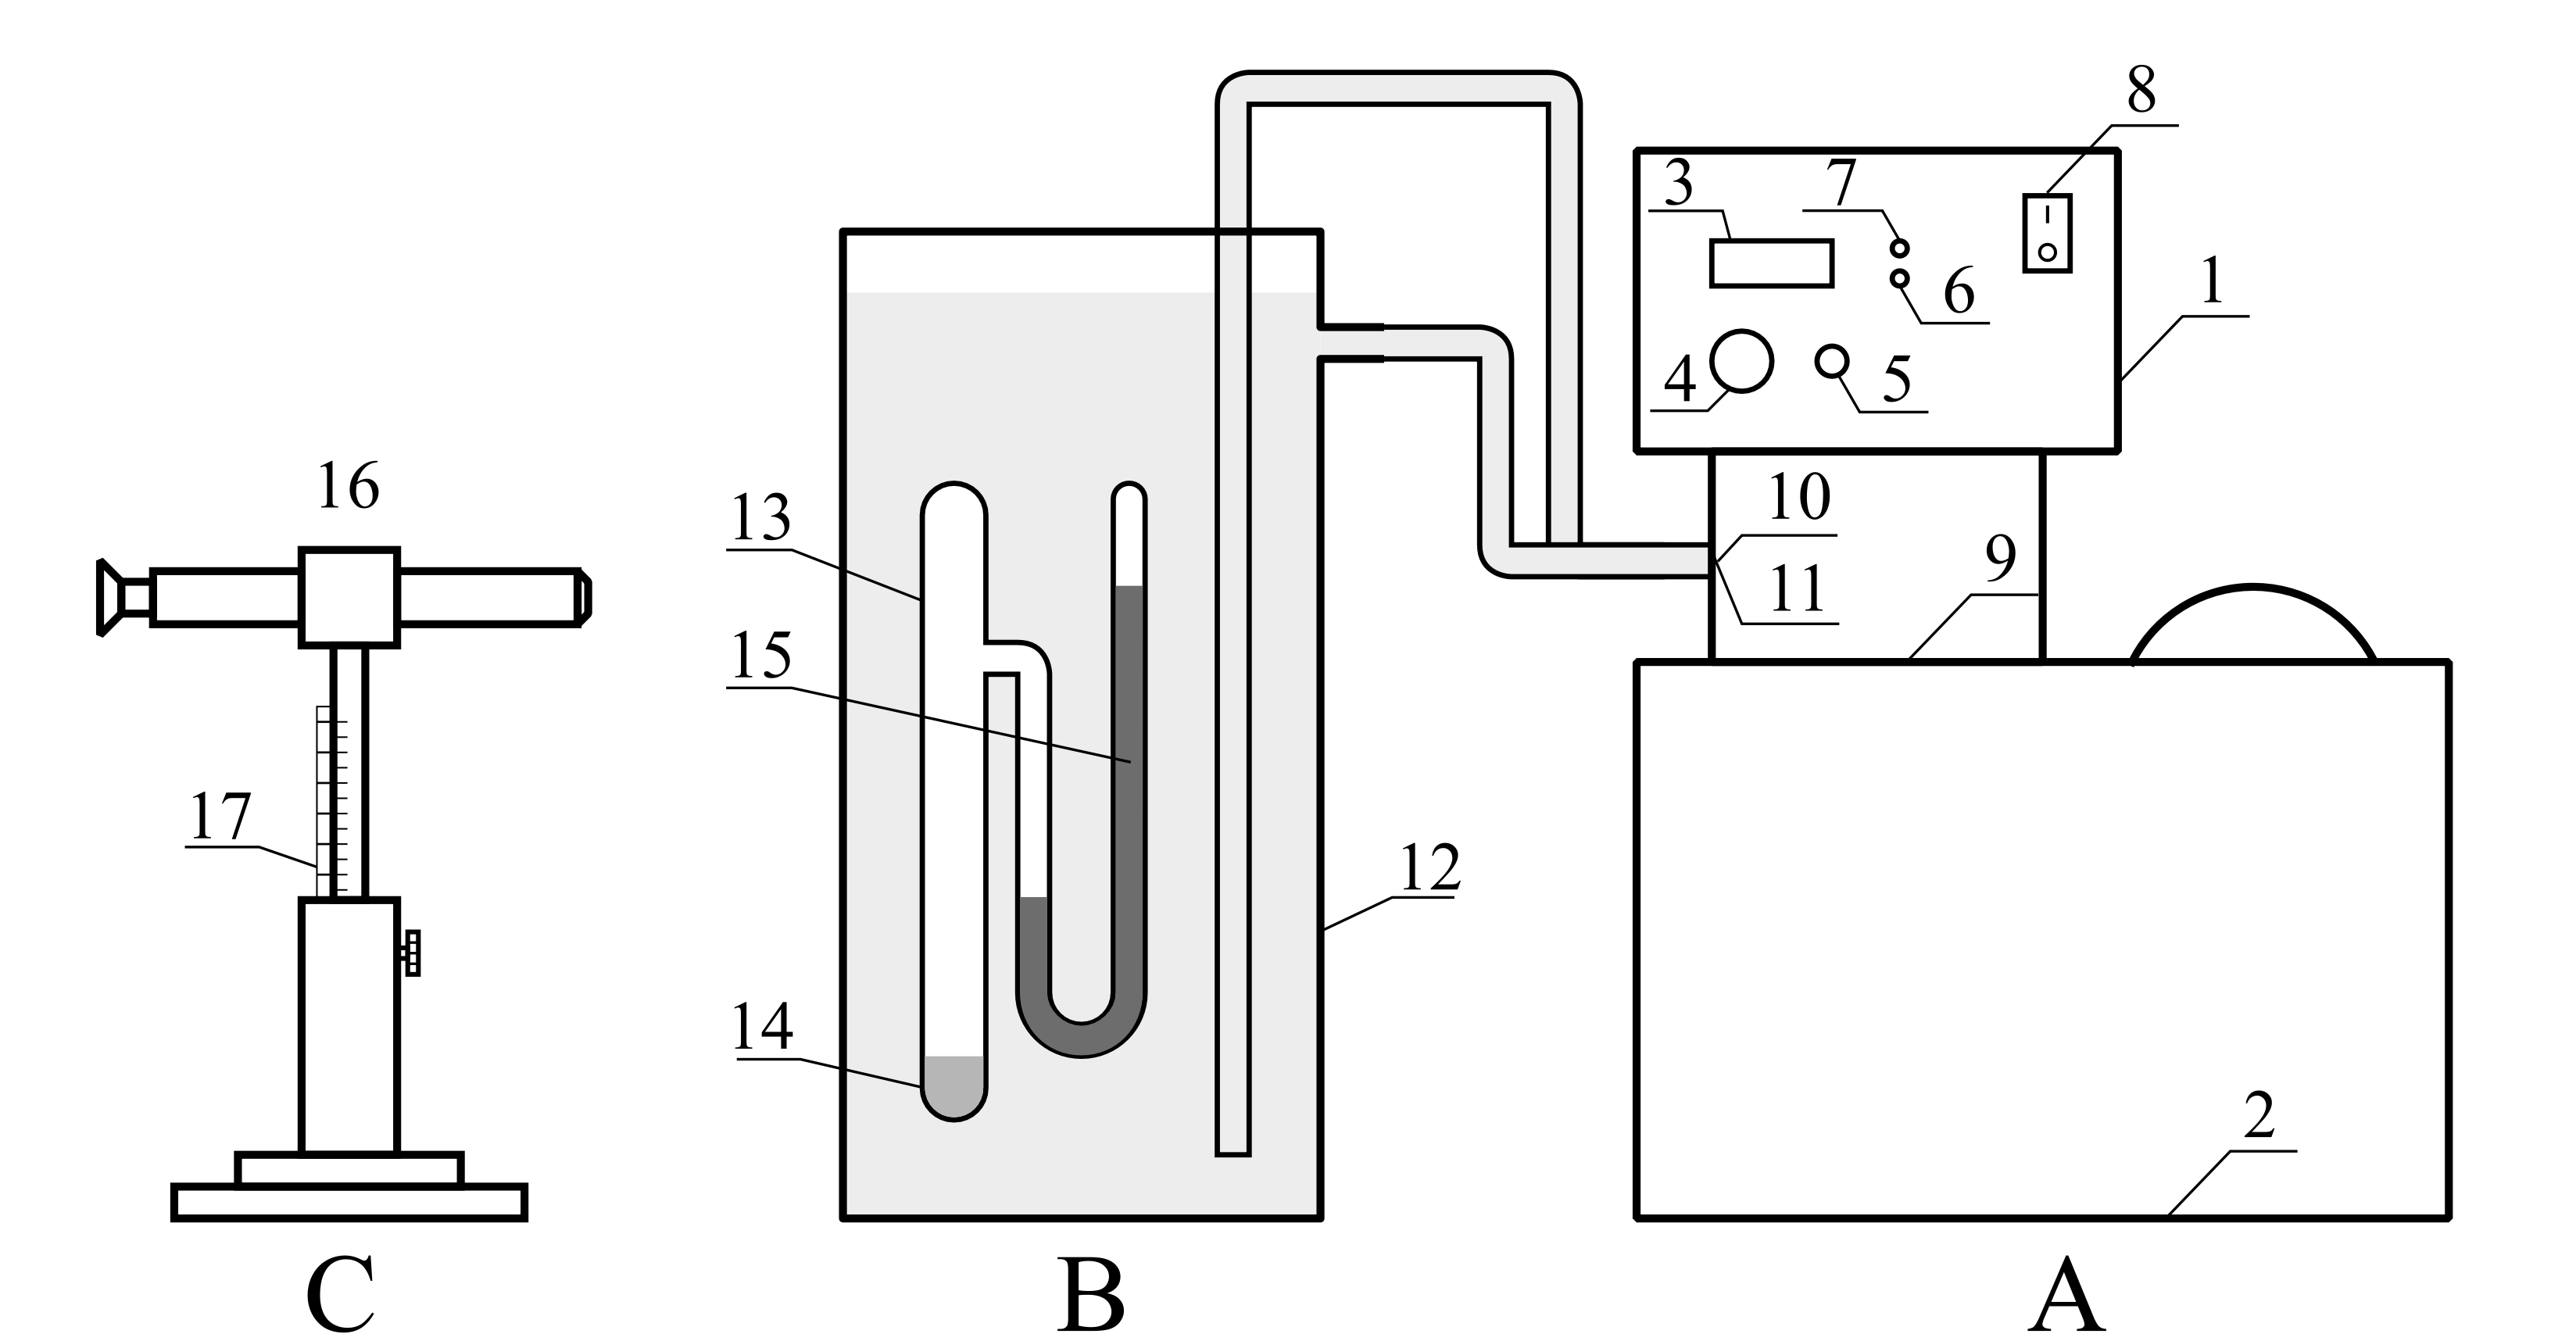
\includegraphics[width=\textwidth]{установка}}
    \caption{Установка для определения давления насыщенных паров.}
    \label{установка}
\end{figure}
\paragraph{}
Измерения проводятся на установке, изображенной на рис. \ref{установка}. С помощью термостата A выставляется желаемя температура, и с помощью микроскопа C измеряется положение менисков ртути в U-образном монометре 15. Давление насыщенных паров считается как разность высот менисков ртути.
\paragraph{}
Измерения проводятся в 2 этапа. В начале жидкость нагревается, а потом остужается. Это делается для того, чтобы посмотреть зависит ли давление насыщенных паров только от состояния жидкости или нет.

\section{Методика измерений}

\begin{enumerate}

    \item
    Измерьте разность уровней в ртутном U-образном манометре с помощью микроскопа и температуру по термометру или индикаторному табло.

    \item
    Включите термостат. Если вы работаете со схемой рис. 1, то подогревайте воду в калориметре, пропуская ток через нагреватель. Следите за тем, чтобы воздух всё время перемешивал воду.

    При работе как со схемой рис. 1, так и со схемой рис. 2, через каждый градус измеряйте давление и температуру.

    Продолжайте повышать температуру в течение половины имеющегося у вас времени, чтобы успеть произвести измерения при остывании прибора. Желательно нагреть жидкость до 40-50 °С.

    \item
    Проведите те же измерения при охлаждении жидкости. Установите такой поток воды, чтобы охлаждение шло примерно тем же темпом, что и нагревание.

    \item
    Постройте графики в координатах $T$, $P$ и в координатах $1/T$, $\ln{P}$. На графики нанесите точки, полученные при нагревании и охлаждении жидкости (разными цветами).

    По формуле (\ref{L}) вычислите $L$, пользуясь данными, полученными сначала из одного, а потом из другого графика. Находятся ли результаты в согласии друг с другом? Оцените ошибку измерений. Какой из графиков позволяет найти $L$ с лучшей точностью?

\end{enumerate}

\newpage

\section{Результаты измерений и обработка данных}

\subsection*{Измерения}

Снимем зависимость давления паров спирта в зависимости от температуры, дожидаясь релаксации, сначала при повышении температуры, потом при понижении. Также сохраним табличные данные, указанные на установке.

\bigskip

\begin{minipage}{0.3\textwidth}
    \begin{tabular}{c|c}
\toprule
$t$, $^\circ C$ & $P$, $мм. рт. ст.$ \\
\midrule
23.15 & 46.49 \\
25.26 & 53.58 \\
27.30 & 59.79 \\
29.24 & 66.75 \\
31.24 & 75.64 \\
33.23 & 84.59 \\
35.22 & 94.01 \\
37.19 & 105.04 \\
39.16 & 116.51 \\
\bottomrule
\end{tabular}

    \captionof{table}{Нагрев}\label{нагрев}
\end{minipage}
\begin{minipage}{0.3\textwidth}
    \begin{tabular}{c|c}
\toprule
$t$, $^\circ C$ & $P$, $мм. рт. ст.$ \\
\midrule
37.00 & 101.24 \\
35.01 & 91.06 \\
33.01 & 82.13 \\
31.00 & 73.74 \\
29.01 & 64.97 \\
26.96 & 58.88 \\
\bottomrule
\end{tabular}

    \captionof{table}{Охлаждение}\label{охлаждение}
\end{minipage}
\begin{minipage}{0.3\textwidth}
    \begin{tabular}{c|c}
\toprule
$t$, $^\circ C$ & $P$, $мм. рт. ст.$ \\
\midrule
0 & 12.20 \\
5 & 17.30 \\
10 & 23.60 \\
15 & 32.20 \\
20 & 43.90 \\
25 & 59.00 \\
30 & 78.80 \\
35 & 103.70 \\
40 & 135.30 \\
\bottomrule
\end{tabular}

    \captionof{table}{Табличные}\label{табличные}
\end{minipage}

\subsection*{Графики}

\begin{figure}[h!]
\begin{center}
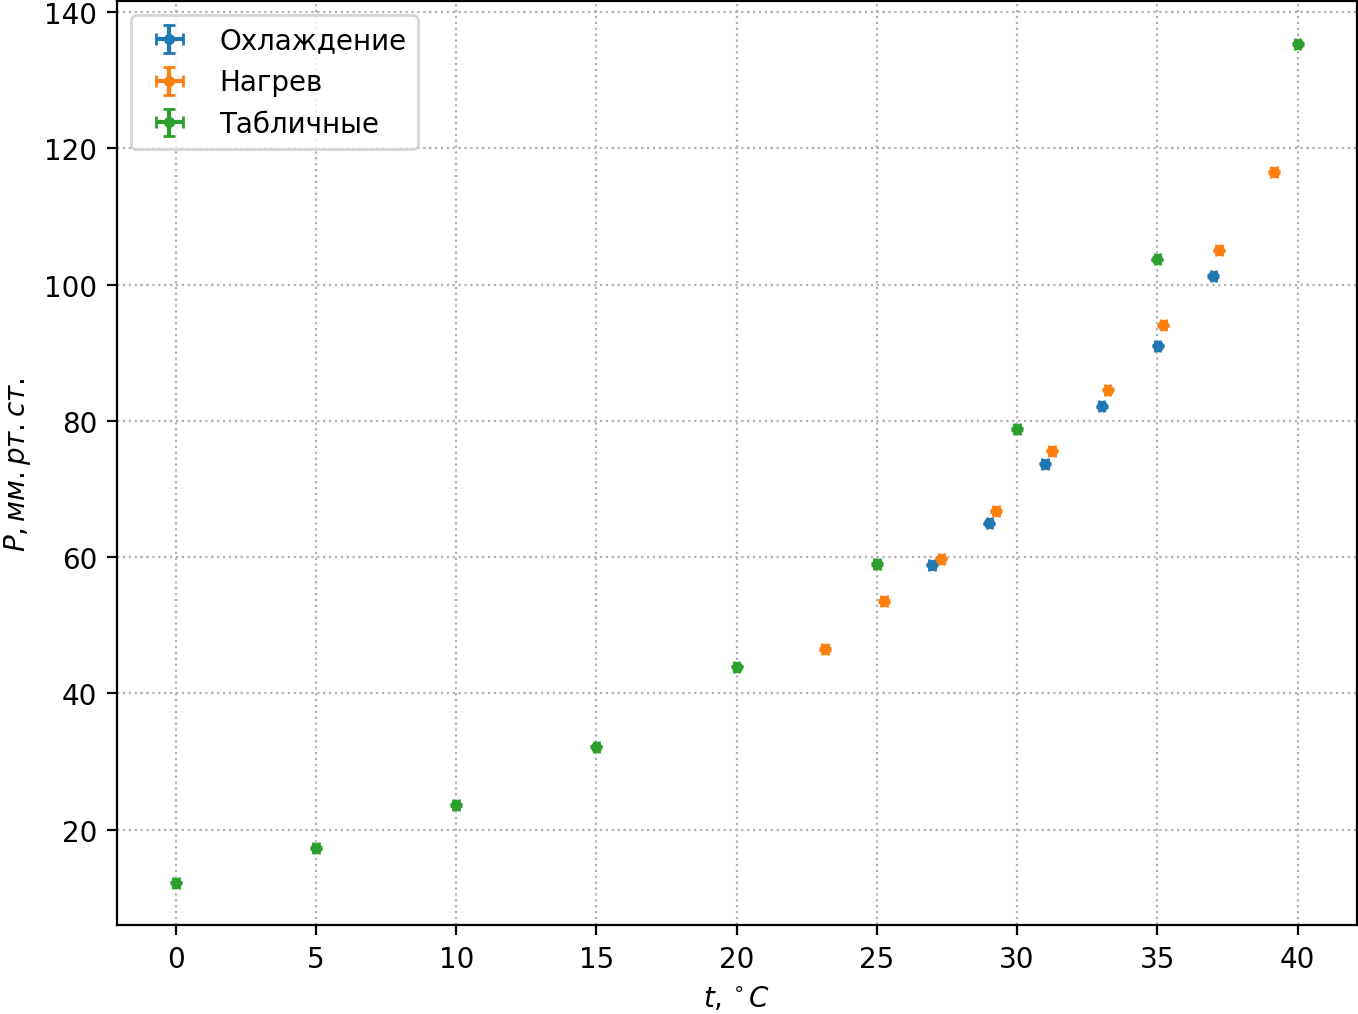
\includegraphics[width=1\textwidth]{P(t).png}
\caption{Зависимость давления от температуры}\label{pt}
\end{center}
\end{figure}

\begin{figure}[h!]
\begin{center}
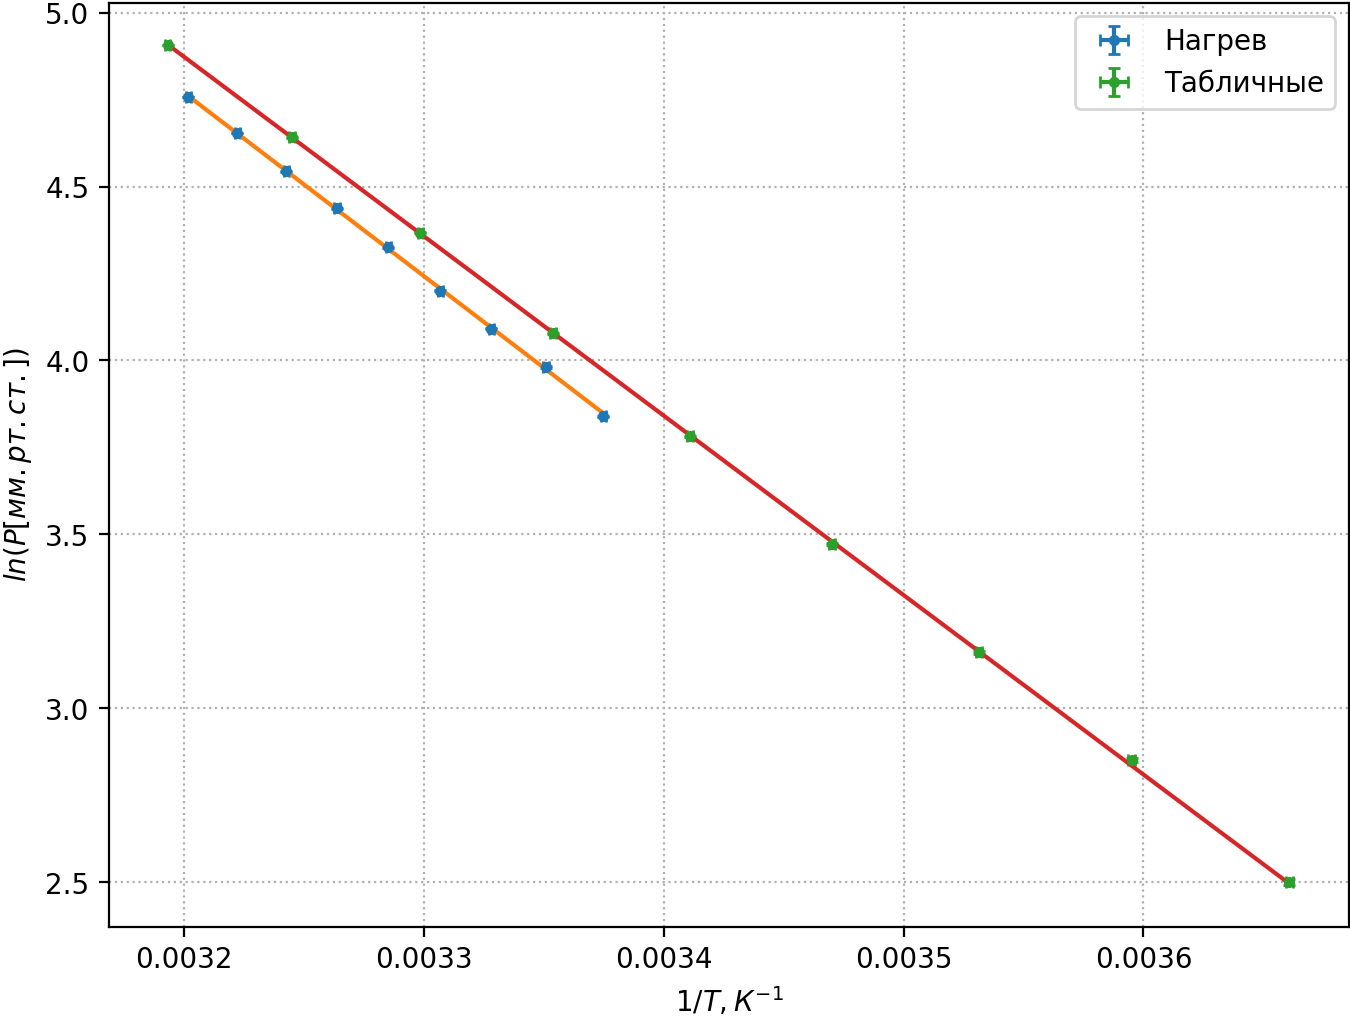
\includegraphics[width=1\textwidth]{lnP(T^-1).png}
\caption{Логарифмическая зависимость}\label{lnpt}
\end{center}
\end{figure}

\subsection*{Теплота испарения спирта}

\subsubsection*{\centering 1 способ}

В каждой точке графика (рис. \ref{pt}) вычислим производную $\frac{dP}{dT}$, а по ней удельную теплоту испраения, используя формулу (\ref{L}). Посчитаем среднее значение и среднеквадратиечское отклонение:
\begin{equation}\label{L1h}
    L^1_{нагр}=950 \pm 29 \ Дж/г

\end{equation}
\begin{equation}\label{L1t}
    L^1_{табл}=935 \pm 13 \ Дж/г

\end{equation}

\subsubsection*{\centering 2 способ}

По графику (рис. \ref{lnpt}) определим коэффициент наклона, а по нему удельную теплоту испраения, используя формулу (\ref{L}):
\begin{equation}\label{L2h}
    L^2_{нагр}=951 \pm 6 \ Дж/г

\end{equation}
\begin{equation}\label{L2t}
    L^2_{табл}=930.4 \pm 2.6 \ Дж/г

\end{equation}

\section{Обсуждение результатов}



\end{document}